\chapter{Results}
In this chapter we present the results of the experiments described in Chapter \ref{chap:models}. These results are presented in the same order as we described the methods and models. Where appropriate we compare our results to previous approaches on the same datasets. Note that the results involving the Yelp Dataset were previously presented in our submission to the Yelp Dataset Challenge.\footnote{https://github.com/sixhobbits/yelp-dataset-2017/} 

\section{Unsupervised Statistical Approaches}
\label{res:unsupervised}

\nocite{cappellato2014clef}

For our unsupervised models, we present results on the training and test sets, as these models did not need to be trained. We compare our results to those achieved in the PAN shared tasks. Note that these results are not directly comparable for several reasons. 

First, the systems that were entered for the shared task were designed to work across various languages, while ours focuses on the English parts of the dataset. Second, the PAN participants were aiming to optimize a so-called ``c@1'' metric, in which systems were penalized less for failing to provide a prediction than for providing the wrong one. That is, systems were encouraged to withhold predictions in the case of difficult or borderline text pairs, while our system generated predictions for all instances. Third, the PAN systems aimed to achieve scores as high as possible, while we attempted to build a system that could be easily interpretable and that could help forensic linguists in manual evaluation.

For the PAN 2014 datasets, we compare ourselves to \citet{khonji2014slightly}, 
who achieved the best overall results and the highest accuracy score for the English novels dataset as well as to \citet{frery2014identification} who achieved the best results for English essays. For PAN 2015, we compare ourselves to \citet{bagnall2015author}, who achieved the best results overall and for the English dataset.

\begin{table}[ht]
\caption{\label{tab:unsupres} The comparative results for our Unsupervised method for the basic and correlation models. We present our highest results using thresholds of 0.75 for both models. Khonji=\citet{khonji2014slightly}, Frery=\citet{frery2014identification}, Bagnal=\citet{bagnall2015author}, tr=train, te=test.}
\begin{center}
\begin{tabular}{lrrrrr} 
\toprule
                       &  \bf Ours & \bf Ours correlation & \bf   Khonji & \bf Frery & \bf Bagnall \\
\midrule
\bf 2014 Novels tr     &    0.82    & 0.65     &          &         &       \\
\bf 2014 Novels te     & 0.70       & 0.46     & 0.75     & 0.61   &       \\
\bf 2014 Essays tr     & 0.61       & 0.42     &          &         &       \\
\bf 2014 Essays te     &   0.68     & 0.52     &  0.59    &  0.72  &       \\
\bf 2015 tr            &   0.68     & 0.57     &          &         &       \\
\bf 2015 te            &    0.66    & 0.65     &          &         & 0.81  \\
\bf All data           &    0.56    & 0.57     &          &         &       \\
\bottomrule
\end{tabular}
\end{center}
\end{table}

The full results for the unsupervised models can be seen in Table \ref{tab:unsupres}. Although we did not beat the winners of the PAN shared tasks with our methods, it is interesting that our results are more stable. Of all the systems submitted for PAN 2014, the ones that did well on the English Essays dataset tended to do badly on the English Novels, and vice-versa, whereas our system achieved similar results on both of these datasets. The PAN 2015 test set is a more challenging dataset as it is deliberately chosen to be cross-topic, as discussed before. \citeauthor{bagnall2015author}'s 
high result on this dataset is from a neural network approach that required nearly 22 hours to run, 
while our system runs in a few minutes. 

The effect of the different thresholds on the accuracy score can be seen in Figure \ref{fig:unsupthresh}. We can see that finding the correct threshold is important. Setting the threshold too low results in the system predicting \textit{same-author} for nearly every instance, and setting it to high results in it predicting \textit{different-author} for nearly every instance. An ongoing challenge for Authorship Attribution tasks that rely on a threshold is to find the correct value for this threshold, as in many real-world cases, as previously discussed, there is no dataset similar enough to the questioned works that can be used to train a classifier and find a correct threshold.

\begin{figure}[ht]
    \label{fig:unsupthresh}
    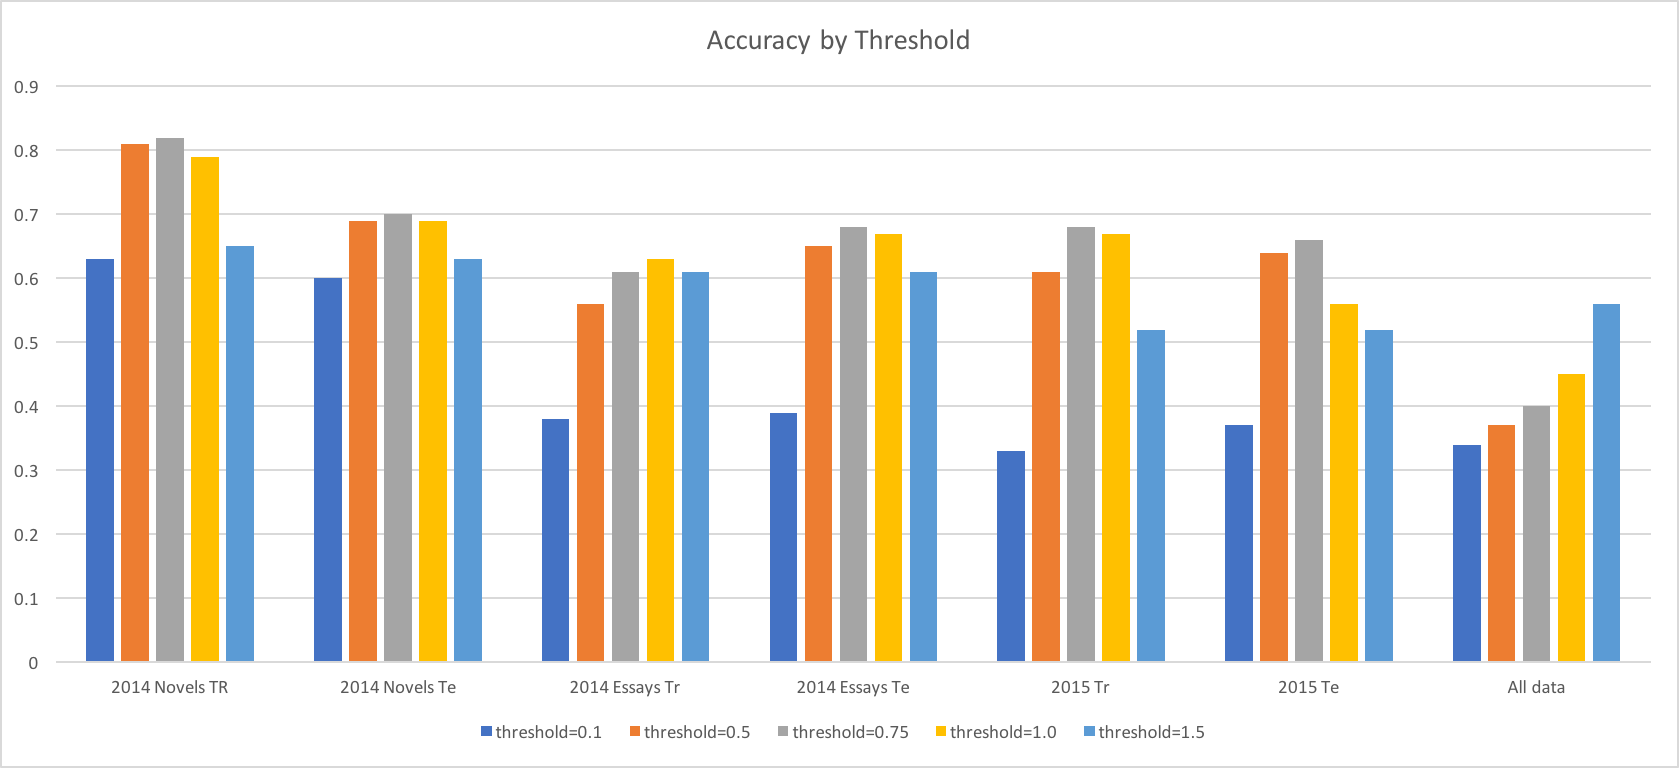
\includegraphics[scale=0.5]{unsupervisedthreshold}
    \caption{The effect of the threshold on the different datasets. Generally setting the threshold too low or too high worsens the results.}
\end{figure}


\section{Support Vector Machine Approaches}
Here we present results for our Support Vector Machine (SVM) approaches for the AID and AV tasks. Unlike the unsupervised approach, the SVM approach did not require language-specific tools, and it scaled well to large datasets. We could therefore test this approach on most of our datasets, but as our Yelp datasets are novel, we cannot compare our results on this dataset to previous attempts.

\subsection{Authorship Identification Tasks}
\label{res:svmaid}
For the AID tasks, we evaluated our models on our Yelp dataset and the C50 dataset. For the former, we have no comparison, as this is the first time that this dataset has been used. However, in Section \ref{res:nn-aid}, we present more discussion about this result when comparing it to our Neural Network model. For the C50 dataset, we compare our results to \citet{houvardas2006ngram}, who introduced the dataset and who presents several results using similar SVM models.

On the Yelp dataset, we achieved an accuracy score of 0.90 using our SVM models. This supports the previous research discussed which showed that Support Vector Machine models are highly effective for many text classification tasks, including Authorship Identification. 

For the C50 dataset, we achieved an accuracy score of 0.72. This is comparable with the work of \citet{houvardas2006ngram}, who reported accuracy scores ranging from 0.69 to 0.74 for various feature selection methods and n-gram ranges.

The fact that we achieved lower scores on the C50 dataset than on the Yelp dataset is interesting because there was more training and test text available in the C50 dataset than the subset of the Yelp dataset that we used. This suggests that authors who write freely on the internet are easier to identify by their writing style than journalists who have been trained to write in similar styles (and who have potentially had their text edited for style by editors and proofreaders). 

\subsection{Authorship Verification Tasks}
\label{res:svmav}

For the Authorship Verification tasks, we achieved the results shown in Table \ref{tab:svmav}.

\begin{table}[ht]
\caption{\label{tab:svmav} The comparative results for our Support Vector Machine models. We present accuracy scores alongside our F1 scores in order to be able to compare to previous high scores at PAN. \textit{B/K} is \citet{bagnall2015author} for 2015 datasets and \citet{khonji2014slightly} for 2014 datasets. ``Yelp short'' and ``Yelp long'' refer to the datasets summarized in Table \ref{verdata-table}}.
\begin{center}
\begin{tabular}{lrrr} 
\toprule
                       &  \bf F1 &    \bf Acc & \bf B/K Acc. \\
\midrule
\bf 2014 en Novels tr     &   0.72     & 0.72   &          \\
\bf 2014 en Novels te     &   0.63     & 0.64   &   0.75    \\
\bf 2014 en Essays tr     &   0.61     & 0.61   &           \\
\bf 2014 en Essays te     &   0.58     & 0.58   &   0.59   \\
\bf 2014 nl Reviews tr     &   0.62    & 0.62  &           \\
\bf 2014 nl Reviews te     &   0.38    & 0.52  &    0.74   \\
\bf 2014 nl Essays tr     &   0.69     & 0.68  &           \\
\bf 2014 nl Essays te     &   0.66     & 0.65  &   0.91    \\
\bf 2014 gr tr             &   0.50    & 0.52  &           \\
\bf 2014 gr te             &   0.47    & 0.51  &   0.89    \\
\bf 2014 es tr             &   0.62    & 0.64  &           \\
\bf 2014 es te             &   0.67    & 0.69  &      0.90 \\
\bf 2015 en tr             &   0.82    & 0.82  &         \\
\bf 2015 en te             &   0.58    & 0.61  &    0.81 \\
\bf 2015 nl tr             &   0.71    & 0.71  &         \\
\bf 2015 nl te             &   0.64    & 0.64  &   0.70  \\
\bf 2015 gr tr             &   0.56    & 0.59  &         \\
\bf 2015 gr te             &   0.57    & 0.57  &    0.88 \\
\bf 2015 es tr             &   0.59    & 0.61  &         \\
\bf 2015 es te             &   0.33    & 0.50  &    0.89 \\
\bf Yelp short             &           & 0.92  &         \\
\bf Yelp long              &           & 0.95  &         \\ 
\hline
\end{tabular}
\end{center}
\end{table}

For the PAN datasets, we failed to achieve higher scores than those achieved by previous PAN winners. However, our method achieved above baseline results for nearly all subsets of PAN and required no tuning or modification for the different datasets. It was also substantially more efficient than the winning PAN models, requiring only a few minutes to run instead of the run times of more than a day reported by the top PAN participants \cite{stamatatos2015overview}.

For the Yelp datasets, we can see that shorter texts are more difficult to accurately classify, even though we had more examples to train on (71\,300 and 38\,900 respectively). However, in both cases our novel approach achieved very high results. As discussed before, these results are especially interesting as the authors in the test set are disjoint from those in the training set (in fact, no author is represented more than once). It is impressive that even using a simple approach, a supervised classifier is able to make meaningful decisions about authors that it has not seen examples of during the training phase.

Although we still need a fair amount of text for each known author, this is far less than what is needed to achieve reasonable results in an identification task. As mentioned before, the verification task can be used a stepping-stone to solve many other authorship attribution tasks, including identification. We could, for example, do pairwise comparisons across all reviews in a corpus to find the likelihood of a single author using multiple accounts, or do a pairwise comparison of all the reviews associated with a single username to find out if it is likely that more than one person uses that account.


\section{Neural Network Approaches}
In this section we present our results on the AID tasks and AV tasks for our Neural Network models. First we present our results on the AID tasks using our character-level language models. This is followed by our results on the AV tasks using Siamese Neural Network models.

\subsection{Authorship Identification Tasks}
\label{res:nn-aid}
This was the most computationally expensive part of our work, as we needed to train an author-specific language model for each candidate author, and then evaluate each test text against each language model. To train and evaluate the models in a reasonalbe amount of time, we used a cloud machine with four virtual CPUs, 61 GiB of RAM and an NVIDIA K80 GPU with 2 496 parallel processing cores and 12 GiB of GPU memory. Even with this extra compute capacity, this experiment took approximately 15 hours to run, substantially longer than our other experiments. Due to time and computate capacity limitations, we therefore present results only against a single dataset, namely the Yelp dataset that we introduced as part of our work.

We achieved an accuracy score of 0.90 on the Yelp dataset. As this is the first time that this dataset has been used for Authorship Identification, we cannot present any comparitive results to previous attempts or models. However, this was the same score achieved by our SVM model, described above, suggesting that character-level neural language modelling can provide an effective solution to at least some Authorship Attribution tasks, which supports the assertions of \citet{bagnall2015author}. 

\subsection{Authorship Verification Tasks}
\label{res:siamese}

We experimented with our Siamese model using all of the PAN 2014 and PAN 2015 data, across various languages. Because results from this model varied substantially between runs, we present average F1-scores over 10 runs, (where we average the F1 score of the positive and negative classes for each run, and then average this over all runs),
along with the lowest and highest score achieved. We further present averaged accuracies over 10 runs in order to compare to previous PAN results for which F1 scores are not available.

\begin{table}[ht]
\caption{\label{tab:siameseres} The comparative results for our Siamese method, averaged over 10 runs. We present accuracy scores alongside our F1 scores in order to be able to compare to previous high scores at PAN. \textit{B/K} is \citet{bagnall2015author} for 2015 datasets and \citet{khonji2014slightly} for 2014 datasets. Note that datasets marked with * were used to tune the models and the results should not be taken as indicative of evaluation.}
\begin{center}
\begin{tabular}{lrrrrr} 
\toprule
                       &  \bf Avg F1 & \bf Min F1 & \bf Max F1 & \bf Avg Acc & \bf B/K Acc. \\
\midrule
\bf 2014 en Novels tr     &   0.64    & 0.54         & 0.70      & 0.66   &          \\
\bf 2014 en Novels te     &   0.59        & 0.52     & 0.61     & 0.64   &   0.75    \\
\bf 2014 en Essays tr     &   0.49       & 0.44      & 0.57     & 0.51   &           \\
\bf 2014 en Essays te     &   0.50     & 0.35        &  0.60    & 0.54   &   0.59   \\
\bf 2014 nl Reviews tr     &   0.34     & 0.33        &  0.38   & 0.50  &           \\
\bf 2014 nl Reviews te     &   0.36     & 0.33        &  0.40    & 0.51  &    0.74   \\
\bf 2014 nl Essays tr     &   0.65     & 0.52        &  0.78    & 0.69  &           \\
\bf 2014 nl Essays te     &   0.59     & 0.50        &  0.69    & 0.64  &   0.91    \\
\bf 2014 gr tr             &   0.40     & 0.33        &  0.49   & 0.53  &           \\
\bf 2014 gr te             &   0.33     & 0.33        &  0.33   & 0.50  &   0.89    \\
\bf 2014 es tr             &   0.46     & 0.42        &  0.49   & 0.53  &           \\
\bf 2014 es te             &   0.40     & 0.37        &  0.44   & 0.53  &      0.90 \\
\bf 2015 en tr*             &   0.82     & 0.76        &  0.91    &  0.82  &         \\
\bf 2015 en te*             &   0.66     & 0.57        &  0.74    &  0.68  &    0.81 \\
\bf 2015 nl tr             &   0.46     & 0.33        &  0.57    &  0.54  &         \\
\bf 2015 nl te             &   0.45     & 0.37        &  0.50    &  0.50  &   0.70  \\
\bf 2015 gr tr             &   0.48     & 0.37        &  0.55    &  0.53  &         \\
\bf 2015 gr te             &   0.35     & 0.33        &  0.37    &  0.50  &    0.88 \\
\bf 2015 es tr             &   0.59     & 0.51        &  0.70    &  0.61  &         \\
\bf 2015 es te             &   0.56     & 0.49        &  0.64    &  0.62  &    0.89 \\
\bottomrule
\end{tabular}
\end{center}
\end{table}

The results are presented in Table \ref{tab:siameseres}, where we can see that the Siamese model did not perform well, underperforming previous PAN winners and in some cases failing to outperform a random baseline. Closer examination of the very low results showed that in these cases the Siamese Network failed to learn anything meaningful from the training dataset, and always or almost always predicted the same label for all test instances. 

We find it interesting that the results for the Siamese Neural Network varied substantially between runs. This could raise some concerns over previous PAN results, in which only a single run was carried out. 
Specifically, the best-performing system in 2014 took over 20 hours to run, and in 2015 the best-performing system needed more than 50 hours to run on the test dataset. This makes it more difficult to test these systems thoroughly over multiple runs.

Overall, we are disappointed that our Siamese Model did not perform better, as believed that this model was the best theoretical fit for task. We are still hopefull that with more experimentation with network architecture, preprocessing, and different datasets that Siamese Models might prove more practically suitable to the AV task.

